\documentclass[11pt]{article} % use larger type; default would be 10pt

\usepackage{graphicx}
\usepackage{amsmath}
\usepackage{fullpage}
\usepackage[parfill]{parskip}

\title{ME 597 Lab 3 Report}
\author{Iain Peet \and Andrei Danaila \and Kevin Kyeong \and Abdel Hamid \and Douche Salam}

\begin{document}
\maketitle

\clearpage

\section{Introduction}
In this lab exercise the Potential Fields and Wavefront planning methods are implemented for planning the trajectory of the robot around a pre-defined obstacle grid map. The methods produce a path that the robot can follow to travel from a given start position towards a pre-defined goal while avoiding known obstacles.

\section{Potential Fields Path Planning}
\subsection{Theory}
The potential fields method is based on the concept of potential function of which value is viewed as energy and gradient is force.  The gradient is a vector $\nabla U(q) = DU(q)^T = [\frac{\partial U}{\partial q_1}, . . . , \frac{\partial U}{\partial q_m}]^T$ which points in the direction that locally maximally increases U \footnote{S. Thrun. \emph{Principles of Robot Motion}. The MIT Press, 2005. (pg.77)}.  This gradient then defines a vector field on an occupancy grid, and directs a robot as if a particle moves in a gradient vector field.

\subsection{Steering}
The robot follows the planned path by steering towards the angle of steepest decent in the potential field map. This allows the robot to calculate the steering angle from any position on the map where the gradient is defined, which is essentially in every free cell in the grid.

Alternatively, we can define waypoints along the path of steepest decent and use the Stanley non-linear steering controller to follow it, but this would be more error prone due to the robot's poor steering which makes it more likely to deviate significantly from the intended path.

\subsection{Results and Observations}
The wavefront method for path planning successfully plotted a map through the obstacles.
The downside of this algorithm was noticed as resulting in substatial increase in steering controller usage
when compared to the wavefront planning method. This was caused to the large number of varying
gradients that the controller tried to follow on its way to the goal.

\begin{figure}[hbt]
 \centering
 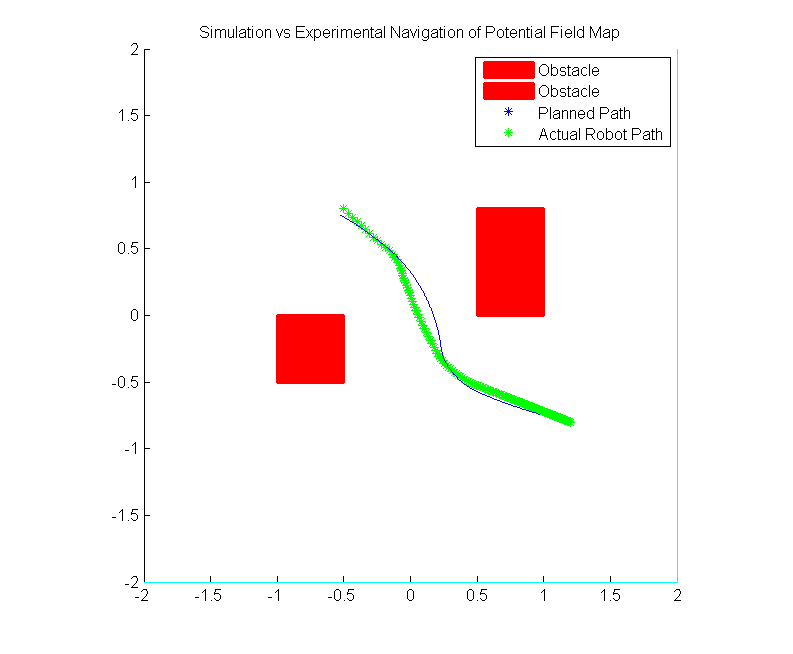
\includegraphics[scale=0.80]{potentialFieldMapNavigation.png}
 \caption{Traversed path through the obstacle map using the potential field algorithm.}
 \label{potFieldMap}
\end{figure}

From \ref{potFieldMap} it is noticed how even though the simulation predicted a sharper turn, 
the robot steering controller could not follow it. Since the robot was not able to perform 
such sharp turns, the volume of the each obstacle was increased in simulation as to provide an artificial
margin of safety to compensate for the lack of steering bandwidth.

\begin{figure}[hbt]
 \centering
 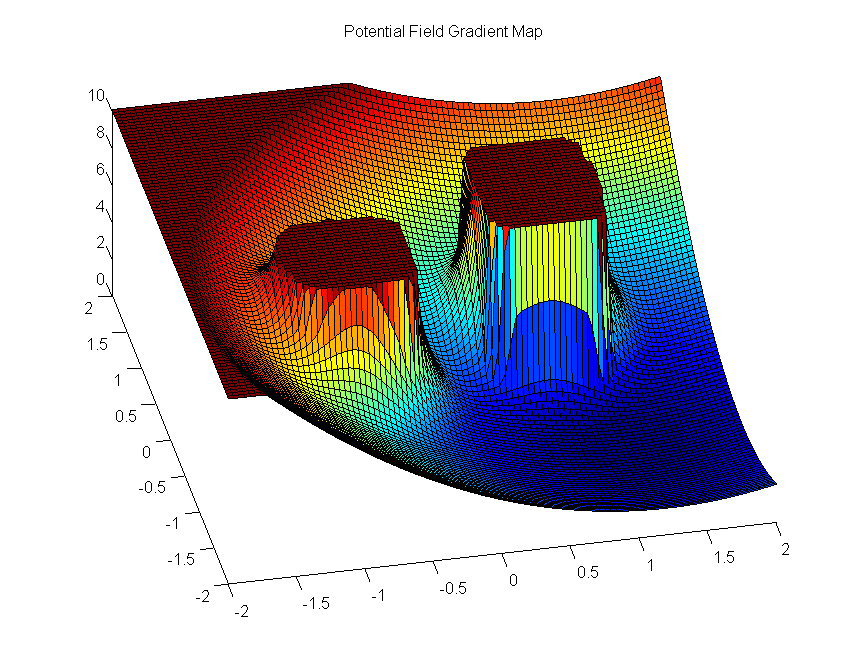
\includegraphics[scale=0.60]{Potential_Field_Surf_Plot.png}
 \caption{Potential field map surface plot.}
 \label{potField_Surf}
\end{figure}


\subsection{Extended Potential Fields}
\section{Wavefront Path Planning}

\subsection{Algorithm Description}
The wavefront planning algorithm is fairly simple in principle.  Cost is propagated outward from the goal, with each cell being assigned a cost one greater than the minimum cost of cells reachable from that cell.  Equivalently, the occupancy grid may be interpreted as a graph where cells are nodes and cells which are reachable from each other are connected by edges.  All edges are assigned a constant cost, and the costs of reaching each cell from the goal are found using Dijkstra's Algorithm.

For this particular application, all cells which are horizonatally, vertically, or diagonally adjacent to a cell are considered to be reachable from that cell.

The wavefront cost computation algorithm is as follows:

\begin{itemize}
 \item Initialize the cost map to 0.
 \item Place the goal cell in the open set, with cost 1.
 \item While there are cells in the open set, \begin{itemize}
  \item Remove a cell from the open set.  This is the current cell.
  \item For each cell reachable from the current cell, \begin{itemize}
    \item If the cell is occupied, move it directly to the closed set, with cost 0.
    \item If the cell is in the unreached set, move it to the open set and assign it a cost one greater than the current open cell.
  \end{itemize}
  \item Place the current cell into the closed set.
 \end{itemize}
\end{itemize}

In the completed cost map, cells which have a cost of zero are obstacles.  For all other cells, the shortest path to the goal requires $n-1$ moves, where $n$ is the cost of the cell.  In order to traverse a shortest path to the goal, the actor must always move to a cell which has lower cost than the current cell.

For the actual robot, a wavefront descent steering controller is defined as follows.  First, the optimal descent direction is computed as follows:

\begin{equation}
\theta_{ref} = tan^{-1}( \frac{ - \frac{\partial C}{\partial y} }{ - \frac{\partial C}{\partial x} } )
\end{equation}

The steering controller is a simple unity feedback controller:
\begin{equation}
\delta = \theta_{ref} - \theta 
\end{equation}

It is likely that the shortest descent paths provided by the wavefront algorithm violate the kinematic constraints of the robot.  The algorithm is adjusted as follows, to allows for path tracking error.  

First, buffer regions are added around obstacles, which are considered to be obstacle region for the purpose of wavefront cost computation.  This ensures that the path provides a certain amount of tolerance for tracking error.

Second, obstacle regions are assigned high cost values, such that their gradient always points to the centre of the obstacle.  This ensures that, if the robot path overshoots into the buffer region, the cost gradient will be defined such that the robot will steer out of the buffer area and back into the 'good' region.

\subsection{Simulation Results}

\begin{figure}
 \centering
 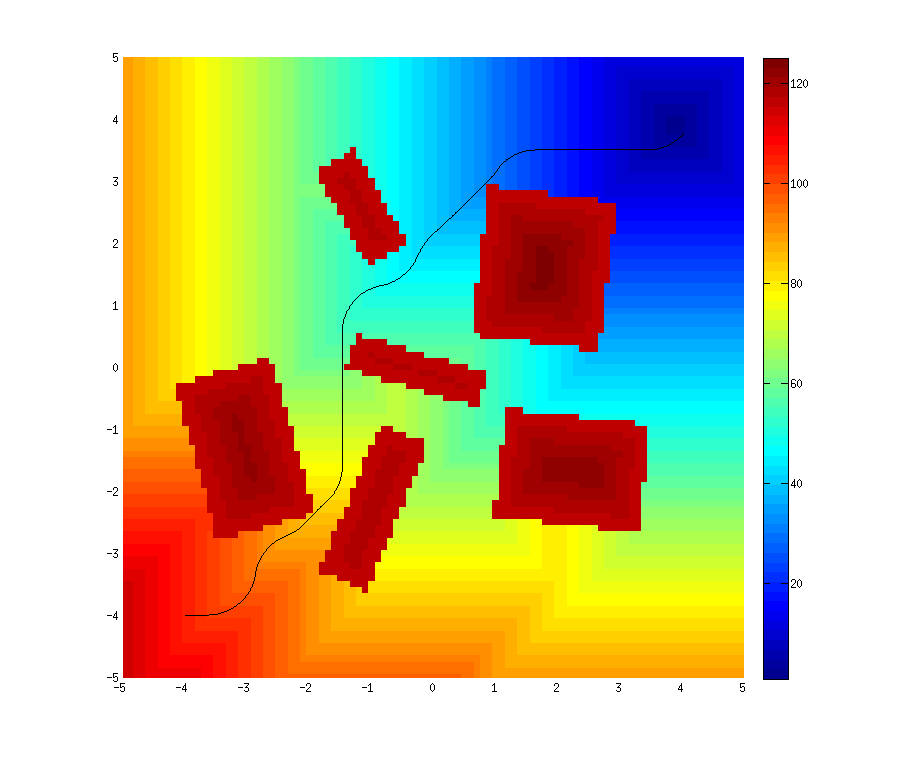
\includegraphics[scale=0.45]{wavefront_good.png}
 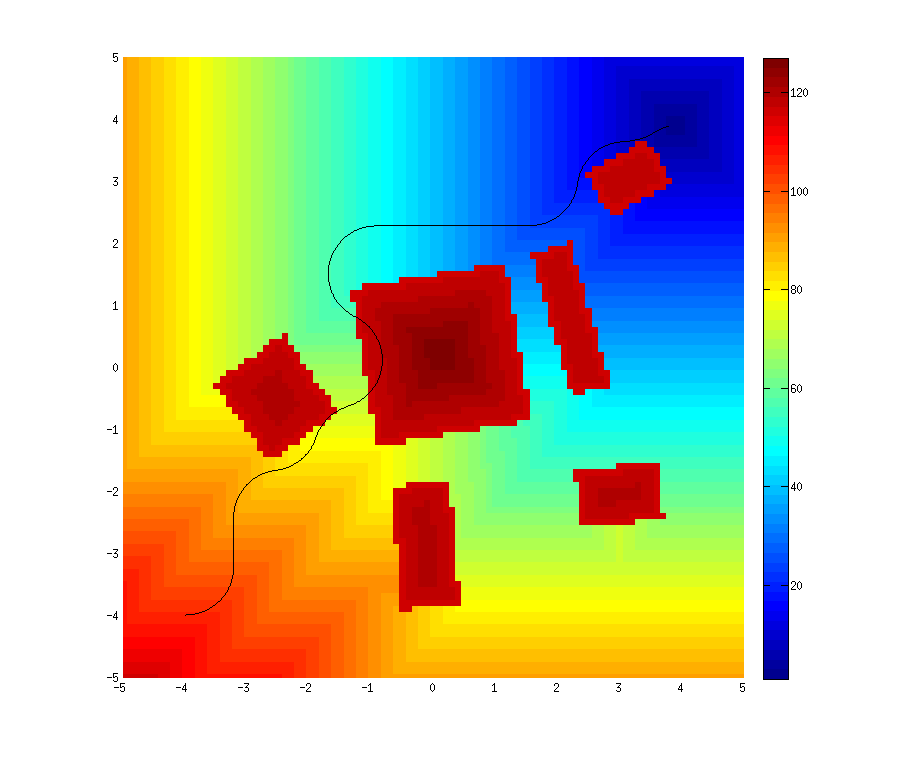
\includegraphics[scale=0.45]{wavefront_kinematic_fail.png}
 \caption{Wavefront costmaps and robot trajectories, for two randomly generated maps.}
 \label{wave_sim}
\end{figure}

Figure \ref{wave_sim} shows simulated results for two different random maps.  Note how, in the second simulation, the robot overshoots the desired trajectories, and recovers as intended.

\clearpage
\subsection{Measured Results}

\begin{figure} [hbt]
 \centering
 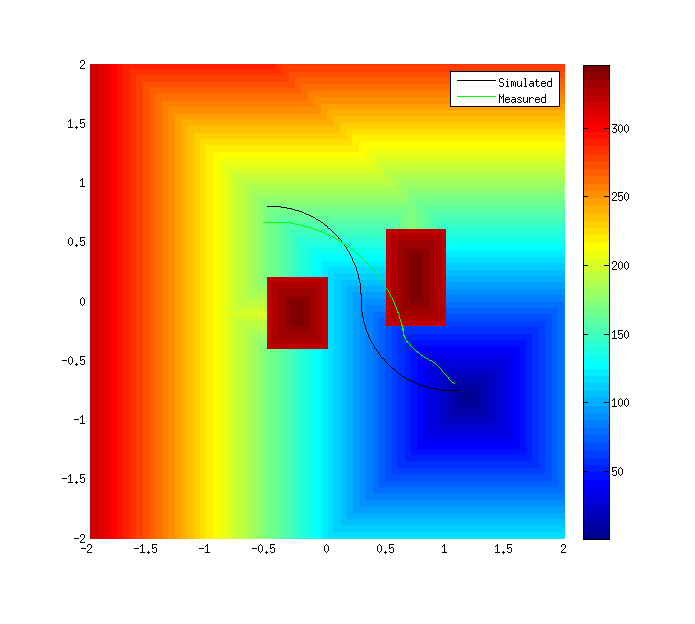
\includegraphics[scale=0.75]{wavefront_meas.png}
 \caption{Simulated and measured robot trajectories, for lab obstacle set-up}
 \label{wave_meas}
\end{figure}

Figure \ref{wave_meas} shows simulated and measured robot trajectories.  The true robot does not steer as sharply as the simulation predicts, which suggests that the modelled maximum steering angle is incorrect.  Otherwise, the measured behaviour appears consistent with expectation.

\subsection{Potential Improvements}
A serious limitation of the wavefront algorithm in this application is the inability to account for the robot's kinematic constraints.  

One possibility would be to extend the occupancy grid to three dimensions, with heading as the third dimension.  The adjacent cells could then be defined to be more plausible state transitions:  in the x and y dimensions, the robot must transition to the neighbor nearest to the current heading co-ordinate.  Heading may remain the same, or transition to adjacent headings.

It is expected that such a problem definition would result in a smoother path, which would be more easily tracked by the steering controller.
\end{document}
